\documentclass[11pt]{article}
\usepackage[utf8]{inputenc}
\usepackage[T1]{fontenc}
\usepackage{amsmath}
\usepackage{amssymb}
\usepackage{multicol}
\usepackage{geometry}
\usepackage{tikz}
\usepackage{enumitem}
\usepackage{xcolor}
\usepackage{titlesec}

% Configurações de layout
\geometry{a4paper, left=1cm, right=1cm, top=0.5cm, bottom=1.2cm}
\setlength{\columnseprule}{0.4pt}

% Cores para títulos
\titleformat{\section}{\normalfont\Large\bfseries\color{blue}}{\thesection}{1em}{}
\titleformat{\subsection}{\normalfont\large\bfseries\color{red}}{\thesubsection}{1em}{}

% Comandos personalizados
\newcommand{\respostaNum}[1]{\textcolor{blue}{\boxed{#1}}}
\newcommand{\respostaTxt}[1]{\textcolor{blue}{#1}}
\newcommand{\resolucao}{\textbf{\textcolor{blue}{Resolução:}}}
\newcommand{\etapa}[1]{\textbf{\textcolor{red}{Etapa #1:}}}
\newcommand{\diretamente}{\textcolor{blue}{Diretamente Proporcional}}
\newcommand{\inversamente}{\textcolor{red}{Inversamente Proporcional}}

\title{\textcolor{green}{Gabarito Comentado: Regra de Três Composta}}
\author{Professor: Jefferson}
\date{}

\begin{document}

\maketitle
\vspace{-1cm}

\begin{multicols}{2}

\section*{Instruções}
\textbf{Verifique suas respostas e estude as resoluções comentadas.}

\section*{Gabarito - Exercícios Propostos}

\begin{enumerate}[leftmargin=*]

\item \textbf{(Produção)} Se 4 impressoras iguais produzem 800 panfletos em 2 horas, quantos panfletos 6 impressoras produzirão em 5 horas?

\resolucao

\textbf{\textcolor{red}{Etapa 1:}} Montar a tabela

\[
\begin{array}{c|c|c}
\text{Impressoras} & \text{Horas} & \text{Panfletos} \\
\hline
4 & 2 & 800 \\
6 & 5 & x
\end{array}
\]

\textbf{\textcolor{red}{Etapa 2:}} Analisar as proporções (em relação aos panfletos)

\begin{itemize}
    \item Impressoras $\times$ Panfletos: Mais impressoras, mais panfletos $\Rightarrow$ \diretamente
    \item Horas $\times$ Panfletos: Mais horas, mais panfletos $\Rightarrow$ \diretamente
\end{itemize}

\textbf{\textcolor{red}{Etapa 3:}} Montar a equação

\[
\frac{800}{x} = \frac{4}{6} \times \frac{2}{5}
\]

\textbf{\textcolor{red}{Etapa 4:}} Calcular

\[
\frac{800}{x} = \frac{4 \times 2}{6 \times 5} = \frac{8}{30} = \frac{4}{15}
\]

\[
4x = 800 \times 15 \Rightarrow 4x = 12000 \Rightarrow x = \frac{12000}{4} = 3000
\]

\respostaTxt{3000 panfletos}

\item \textbf{(Viagem)} Um carro, a uma velocidade média de 80 km/h, percorre um trajeto em 3 horas. Se a velocidade aumentar para 100 km/h, em quanto tempo fará o mesmo percurso?

\resolucao

\textbf{\textcolor{red}{Etapa 1:}} Montar a tabela

\[
\begin{array}{c|c}
\text{Velocidade (km/h)} & \text{Tempo (h)} \\
\hline
80 & 3 \\
100 & x
\end{array}
\]

\textbf{\textcolor{red}{Etapa 2:}} Analisar a proporção

\begin{itemize}
    \item Velocidade $\times$ Tempo: Mais velocidade, menos tempo $\Rightarrow$ \inversamente
\end{itemize}

\textbf{\textcolor{red}{Etapa 3:}} Montar a equação (inverter a razão)

\[
\frac{3}{x} = \frac{100}{80}
\]

\textbf{\textcolor{red}{Etapa 4:}} Calcular

\[
\frac{3}{x} = \frac{100}{80} = \frac{5}{4} \Rightarrow 5x = 12 \Rightarrow x = \frac{12}{5} = 2,4
\]

\respostaTxt{2,4 horas} (ou 2h24min)

\item \textbf{(Obra)} 8 pedreiros constroem um muro de 200 m² em 12 dias. Quantos pedreiros seriam necessários para construir 300 m² em 8 dias?

\resolucao

\textbf{\textcolor{red}{Etapa 1:}} Montar a tabela

\[
\begin{array}{c|c|c}
\text{Pedreiros} & \text{Muro (m²)} & \text{Dias} \\
\hline
8 & 200 & 12 \\
x & 300 & 8
\end{array}
\]

\textbf{\textcolor{red}{Etapa 2:}} Analisar as proporções (em relação aos pedreiros)

\begin{itemize}
    \item Muro $\times$ Pedreiros: Mais muro, mais pedreiros $\Rightarrow$ \diretamente
    \item Dias $\times$ Pedreiros: Menos dias, mais pedreiros $\Rightarrow$ \inversamente
\end{itemize}

\textbf{\textcolor{red}{Etapa 3:}} Montar a equação

\[
\frac{8}{x} = \frac{200}{300} \times \frac{8}{12}
\]

\textbf{\textcolor{red}{Etapa 4:}} Calcular

\[
\frac{8}{x} = \frac{2}{3} \times \frac{2}{3} = \frac{4}{9}
\]

\[
4x = 72 \Rightarrow x = \frac{72}{4} = 18
\]

\respostaTxt{18 pedreiros}

\item \textbf{(Ração)} Em um hotel com 20 hóspedes, há comida suficiente para 15 dias. Se chegarem mais 5 hóspedes, mantendo a mesma quantidade de comida, por quantos dias a comida durará?

\resolucao

\textbf{\textcolor{red}{Etapa 1:}} Montar a tabela

\[
\begin{array}{c|c}
\text{Hóspedes} & \text{Dias} \\
\hline
20 & 15 \\
25 & x
\end{array}
\]

\textbf{\textcolor{red}{Etapa 2:}} Analisar a proporção

\begin{itemize}
    \item Hóspedes $\times$ Dias: Mais hóspedes, menos dias $\Rightarrow$ \inversamente
\end{itemize}

\textbf{\textcolor{red}{Etapa 3:}} Montar a equação

\[
\frac{15}{x} = \frac{25}{20}
\]

\textbf{\textcolor{red}{Etapa 4:}} Calcular

\[
\frac{15}{x} = \frac{25}{20} = \frac{5}{4} \Rightarrow 5x = 60 \Rightarrow x = \frac{60}{5} = 12
\]

\respostaTxt{12 dias}

\item \textbf{(Complexo)} 15 operários, trabalhando 9 horas por dia, produzem 1200 peças em 20 dias. Quantas horas por dia deverão trabalhar 18 operários para produzir 1800 peças em 15 dias?

\resolucao

\textbf{\textcolor{red}{Etapa 1:}} Montar a tabela

\[
\begin{array}{c|c|c|c}
\text{Operários} & \text{horas/dia} & \text{Dias} & \text{Peças} \\
\hline
15 & 9 & 20 & 1200 \\
18 & x & 15 & 1800
\end{array}
\]

\textbf{\textcolor{red}{Etapa 2:}} Analisar as proporções (em relação a horas/dia)

\begin{itemize}
    \item Operários $\times$ horas/dia: Mais operários, menos horas/dia $\Rightarrow$ \inversamente
    \item Dias $\times$ horas/dia: Menos dias, mais horas/dia $\Rightarrow$ \inversamente
    \item Peças $\times$ horas/dia: Mais peças, mais horas/dia $\Rightarrow$ \diretamente
\end{itemize}

\textbf{\textcolor{red}{Etapa 3:}} Montar a equação

\[
\frac{9}{x} = \frac{18}{15} \times \frac{15}{20} \times \frac{1200}{1800}
\]

\textbf{\textcolor{red}{Etapa 4:}} Simplificar e calcular

\[
\frac{18}{15} = \frac{6}{5}, \quad \frac{15}{20} = \frac{3}{4}, \quad \frac{1200}{1800} = \frac{2}{3}
\]

\[
\frac{9}{x} = \frac{6}{5} \times \frac{3}{4} \times \frac{2}{3} = \frac{36}{60} = \frac{3}{5}
\]

\[
3x = 45 \Rightarrow x = \frac{45}{3} = 15
\]

\respostaTxt{15 horas por dia}

\item \textbf{(Torres)} Uma torneira enche um tanque em 6 horas. Duas torneiras iguais a essa enchem o mesmo tanque em quanto tempo?

\resolucao

\textbf{\textcolor{red}{Etapa 1:}} Montar a tabela

\[
\begin{array}{c|c}
\text{Torneiras} & \text{Tempo (h)} \\
\hline
1 & 6 \\
2 & x
\end{array}
\]

\textbf{\textcolor{red}{Etapa 2:}} Analisar a proporção

\begin{itemize}
    \item Torneiras $\times$ Tempo: Mais torneiras, menos tempo $\Rightarrow$ \inversamente
\end{itemize}

\textbf{\textcolor{red}{Etapa 3:}} Montar a equação

\[
\frac{6}{x} = \frac{2}{1}
\]

\textbf{\textcolor{red}{Etapa 4:}} Calcular

\[
2x = 6 \Rightarrow x = \frac{6}{2} = 3
\]

\respostaTxt{3 horas}

\item \textbf{(Custo)} Se 5 costureiras fazem 60 uniformes em 4 dias, quantos uniformes 8 costureiras farão em 6 dias?

\resolucao

\textbf{\textcolor{red}{Etapa 1:}} Montar a tabela

\[
\begin{array}{c|c|c}
\text{Costureiras} & \text{Dias} & \text{Uniformes} \\
\hline
5 & 4 & 60 \\
8 & 6 & x
\end{array}
\]

\textbf{\textcolor{red}{Etapa 2:}} Analisar as proporções (em relação aos uniformes)

\begin{itemize}
    \item Costureiras $\times$ Uniformes: Mais costureiras, mais uniformes $\Rightarrow$ \diretamente
    \item Dias $\times$ Uniformes: Mais dias, mais uniformes $\Rightarrow$ \diretamente
\end{itemize}

\textbf{\textcolor{red}{Etapa 3:}} Montar a equação

\[
\frac{60}{x} = \frac{5}{8} \times \frac{4}{6}
\]

\textbf{\textcolor{red}{Etapa 4:}} Calcular

\[
\frac{60}{x} = \frac{5}{8} \times \frac{2}{3} = \frac{10}{24} = \frac{5}{12}
\]

\[
5x = 720 \Rightarrow x = \frac{720}{5} = 144
\]

\respostaTxt{144 uniformes}

\item \textbf{(Energia)} Em uma usina, 8 geradores consomem 2000 litros de combustível em 5 horas. Quantos litros 5 geradores consumirão em 8 horas?

\resolucao

\textbf{\textcolor{red}{Etapa 1:}} Montar a tabela

\[
\begin{array}{c|c|c}
\text{Geradores} & \text{Horas} & \text{Litros} \\
\hline
8 & 5 & 2000 \\
5 & 8 & x
\end{array}
\]

\textbf{\textcolor{red}{Etapa 2:}} Analisar as proporções (em relação aos litros)

\begin{itemize}
    \item Geradores $\times$ Litros: Menos geradores, menos litros $\Rightarrow$ \diretamente
    \item Horas $\times$ Litros: Mais horas, mais litros $\Rightarrow$ \diretamente
\end{itemize}

\textbf{\textcolor{red}{Etapa 3:}} Montar a equação

\[
\frac{2000}{x} = \frac{8}{5} \times \frac{5}{8}
\]

\textbf{\textcolor{red}{Etapa 4:}} Calcular

\[
\frac{2000}{x} = \frac{8}{5} \times \frac{5}{8} = 1
\]

\[
x = 2000
\]

\respostaTxt{2000 litros}

\item \textbf{(Digitação)} 3 digitadores digitam 12 páginas em 2 horas. Quantos digitadores são necessários para digitar 30 páginas em 3 horas?

\resolucao

\textbf{\textcolor{red}{Etapa 1:}} Montar a tabela

\[
\begin{array}{c|c|c}
\text{Digitadores} & \text{Páginas} & \text{Horas} \\
\hline
3 & 12 & 2 \\
x & 30 & 3
\end{array}
\]

\textbf{\textcolor{red}{Etapa 2:}} Analisar as proporções (em relação aos digitadores)

\begin{itemize}
    \item Páginas $\times$ Digitadores: Mais páginas, mais digitadores $\Rightarrow$ \diretamente
    \item Horas $\times$ Digitadores: Mais horas, menos digitadores $\Rightarrow$ \inversamente
\end{itemize}

\textbf{\textcolor{red}{Etapa 3:}} Montar a equação

\[
\frac{3}{x} = \frac{12}{30} \times \frac{3}{2}
\]

\textbf{\textcolor{red}{Etapa 4:}} Calcular

\[
\frac{3}{x} = \frac{2}{5} \times \frac{3}{2} = \frac{6}{10} = \frac{3}{5}
\]

\[
3x = 15 \Rightarrow x = \frac{15}{3} = 5
\]

\respostaTxt{5 digitadores}

\item \textbf{(Desafio)} Para asfaltar 30 km de uma estrada, 15 trabalhadores levam 18 dias. Após 6 dias de trabalho, 5 trabalhadores adoeceram e não puderam continuar. Considerando que o ritmo de trabalho se manteve, quantos dias a mais serão necessários para concluir a obra?

\resolucao

\textbf{\textcolor{red}{Etapa 1:}} Calcular o trabalho já realizado

Trabalho total: 30 km em 18 dias com 15 trabalhadores

\textbf{\textcolor{red}{Etapa 2:}} Calcular a produção diária por trabalhador

Em 18 dias, 15 trabalhadores fazem 30 km

Em 1 dia, 15 trabalhadores fazem $\frac{30}{18} = \frac{5}{3}$ km

Em 1 dia, 1 trabalhador faz $\frac{5/3}{15} = \frac{5}{45} = \frac{1}{9}$ km

\textbf{\textcolor{red}{Etapa 3:}} Calcular o que foi feito em 6 dias

Em 6 dias com 15 trabalhadores: $6 \times 15 \times \frac{1}{9} = 6 \times \frac{15}{9} = 6 \times \frac{5}{3} = 10$ km

\textbf{\textcolor{red}{Etapa 4:}} Calcular o que falta

Falta: $30 - 10 = 20$ km

\textbf{\textcolor{red}{Etapa 5:}} Calcular com os trabalhadores restantes

Trabalhadores restantes: $15 - 5 = 10$

Produção diária com 10 trabalhadores: $10 \times \frac{1}{9} = \frac{10}{9}$ km/dia

\textbf{\textcolor{red}{Etapa 6:}} Calcular dias necessários para o restante

Dias restantes = $\frac{20}{10/9} = 20 \times \frac{9}{10} = 18$ dias

\textbf{\textcolor{red}{Etapa 7:}} Calcular dias a mais

Dias originalmente previstos para o restante: 18 dias totais - 6 já passados = 12 dias

Dias a mais = $18 - 12 = 6$

\respostaTxt{6 dias a mais}

\end{enumerate}

\section*{Resumo das Fórmulas}

\begin{center}
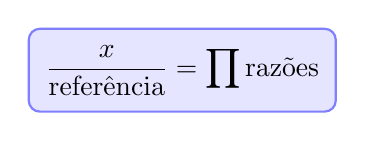
\begin{tikzpicture}
\node[rectangle, fill=blue!10, rounded corners, inner sep=6pt, draw=blue!50, thick] (box) {
$\displaystyle \frac{x}{\text{referência}} = \prod \text{razões}$
};
\end{tikzpicture}

\vspace{0.2cm}

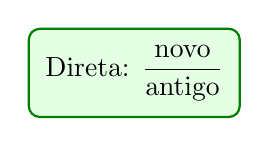
\begin{tikzpicture}
\node[rectangle, fill=green!10, rounded corners, inner sep=6pt, draw=green!50!black, thick] (box) {
$\displaystyle \text{Direta: } \frac{\text{novo}}{\text{antigo}}$
};
\end{tikzpicture}

\vspace{0.2cm}

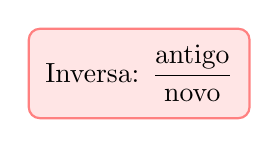
\begin{tikzpicture}
\node[rectangle, fill=red!10, rounded corners, inner sep=6pt, draw=red!50, thick] (box) {
$\displaystyle \text{Inversa: } \frac{\text{antigo}}{\text{novo}}$
};
\end{tikzpicture}
\end{center}

\vspace{0.3cm}
\textcolor{blue}{\textbf{Legenda:}} 
\begin{itemize}
\item \textcolor{blue}{Respostas numéricas:} \respostaTxt{exemplo}
\item \textcolor{blue}{Respostas textuais:} \textcolor{blue}{exemplo}
\end{itemize}

\vspace{0.3cm}
\textcolor{red}{\textbf{Passo a passo da resolução:}}
\begin{enumerate}
    \item \textcolor{blue}{Montar a tabela com todas as grandezas}
    \item \textcolor{blue}{Isolar a grandeza com a incógnita}
    \item \textcolor{blue}{Comparar cada grandeza com a da incógnita}
    \item \textcolor{blue}{Identificar se é direta ou inversa}
    \item \textcolor{blue}{Montar a proporção}
    \item \textcolor{blue}{Simplificar e calcular}
\end{enumerate}

\end{multicols}

\end{document}
